\subsection{Questions}

In order for the interview to go smoothly it is important to define the questions beforehand. The questions will be based on the research framework and the evaluation criteria. The interviews will be conducted by Jessie Liauw A Fong and the interviewee will be a software architect.

Questions about how they view software architecture:
\begin{itemize}
  \item What is software architecture?
  \item What is your company the main job of a software architect?
  \item Which with kind of architectures have you worked?
  \item What is the biggest pitfall when implementing a new architecture?
  \item How do you decide which architecture is best of a certain project?
  \item What is the architecture that you implement in most of your projects? (Frontend and backend)
\end{itemize}

Questions about how they view modularity:
\begin{itemize}
  \item What is the first thing that you think of when I say modular architecture?
  \item What are the most upcoming architectures that are focused on modularity in your opinion?
  \item Which programming languages do you think compliments a modular architecture best?
  \item
\end{itemize}

Questions about the chosen architecture and method:
\begin{itemize}
  \item What do you think of the image about how I went my way in choosing the right architecture?
  \item What is your opinion about domain driven design
  \item Have you ever heard of modular monolith
\end{itemize}

\begin{figure}[H]
	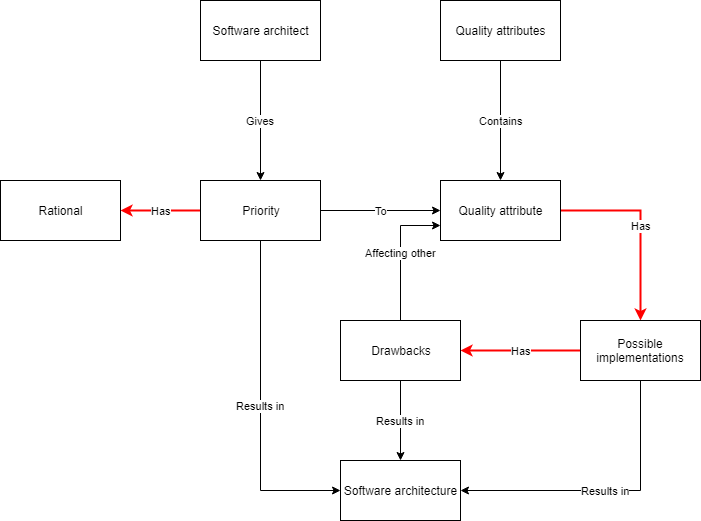
\includegraphics[width=\linewidth]{creating_architecture.png}
	\caption{How a software architecture is chosen}
\end{figure}

\subsection{Interview with Joris}
\subsection{Interview with Joris}

Jessie: Na mijn eerste vraag aan jou is eigenlijk. Wat is in jouw ogen software architectuur?

Joris: Nou dan hadden weer meteen ook. Heb je een half uurtje?

Jessie: Als je het zo beknopt mogelijk zou moeten uitleggen aan iemand.

Joris: Dan is het sofware architectuur een model van hoe een stuk software geimplementeerd is. Het is een soort abstractie. Als je kijkt naar de architectuur van de auto bijvoorbeeld, de motor bestuur en de deur. Op dat niveau zo kun je ook de software kijken. Software verdeel je ook op een bepaalde manier in min of meer onafhankelijke delen en die delen hebben vervolgens de relatie met elkaar. Dus aan het stuur draai gaan de wielen zo. Als ik software dit hier gebeurt, gebeurt er ergens anders iets anders. En architectuur een van de definitie van architectuur is een soort gedeeld model, gedeeld met engineers en de eigenaar van de software. Over hoe die software nou opgedeeld in brokken en hoe die brokken gezamenlijk werken om de functionaliteit geimplementeerd te krijgen.

Jessie: Ja.

Joris: Korter dan dat krijg ik het niet.

Jessie: Nee dat is een goeie beschrijving. En binnen Ximedes, hebben jullie daar iemand die echt alleen op de software architectuur zit?

Joris: Nee, bij ons is er, vrijwel elk team rol van software architect. Typisch, tegelijkertijd ook de meest ervaren developer. Dus bij ons is de architect ook, die bouwt mee. Meestal wordt er op een bepaald niveau wel iets gedocumenteerd over de architectuur. Met name voor mensen die niet in het team zitten dus opdrachtgevers of mensen die nieuw komen. Ik denk dat in de meeste gevallen de architectuur nog veel meer een gedeeld begrip is binnen zo'n team of dat nou echt een los product is. We hebben ook niemand die alleen maar architect is en niet bouwt.

Jessie: Hoe documentaireserie die architectuur?

Joris: Ja dat wisselt. Ook dat wij werken voor verschillende opdrachtgevers die ook zelf verschillende mensen en eisen hebben. De meeste projecten hebben een document, word document bij wijze van spreken of markdown. Vrije teksten en daar wordt in opgeschreven wat mensen. Het is een beetje een soort cirkel definitie maar daar schrijven op wat het team nodig vindt om op te schrijven.

Jessie: Ja.

Joris: Dat dat wisselt heel erg voor detailniveau. Wat ik altijd deed, ik heb zelf ook gearchitect. Je beschrijft het systeem als geheel met de grove delen is sommige. Sommige stukken ga je even de diepte in. Omdat er bijvoorbeeld iets interessants gebeurt if iets niet voor de hand liggend. Want 9 van de 10 keer zeker bij ons geval wij schrijven code van, typisch project van 40000 regels of zo dus dat moet je. Als je naar kijkt moet je toch wel. Het idee is dat we zulke code schrijven dat als je er naar kijkt je het toch wel snapt. Dus dan hoef je niet helemaal te gaan zitten documenteren.

Jessie: Ja.

Joris: Maar goed daar naast zijn er best een aantal klanten vroeger meer dan nu. Die het heel formeel gedocumenteerd willen hebben. Dingen als uml unified modeling language. We deden het al niet veel en we doen het nu nog minder, omdat klanten het niet meer nodig vinden.

Jessie: En als je dan kijkt naar de verschillen architecturen die binnen Ximedes worden gebruikt. Eelke zijn dat en waarom is daar voor gekozen?

Joris: Ja. Ik denk met afstand de meest voorkomende architectuur is een monoliet. Java of tegenwoordig kotlin, maar een web applicaite op JVM. Die communiceert met relationele databases. En dat of een server sided gerenderde html ui heeft of rich client zoals react, angular of vue die communiceert via de rest api. Ik denk dat dat 80 procent van de projecten zijn. En dat kiezen we omdat we, we geloven er heel erg dat je dingen zo eenvoudig mogelijk moet maken. En dat is een kunst, daar zijn geen harde regels voor maar door de bank genomen is een monoliet voor developers, voor beheerders, voor eigenaars. Eenvoudiger dan een microservices architectuur bijvoorbeeld. En dus als je kijkt naar microservices als alternatief van een monoliet. Dat is nogal wat investeringen die inkomt. Het wordt complex op te bouwen, complex om te deployen. Het lost een hele specifieke set aan problemen op die lang niet elk klant heeft. Voor de de de lood en de performance en de security die wij nodig hebben is een monoliet uitstekend. Dus dat is een beetje de defacto standaard. En wat je vervolgens ziet is dat je per project per klant daarin wordt afgeweken daar waar het nodig is en daar waar het zinnig is. Dus soms worden systemen in 2 delen op in 3 delen of 20 delen opgesplitst.

Jessie: Je wilt je kijkt gewoon naar bijvoorbeeld. Als er 1 deel is wat eigenlijk 9 procent van de loadopvang dan wil je eigenlijk alleen deel onderscheiden.

Joris: Ja, bijvoorbeeld.

Jessie: Dat je die makkelijker kan delen en dat de rest van de applicatie in een instance kan draaien.

Joris: Ja bijvoorbeeld, security is bijvoorbeeld een ander ding. Waarbij je zo min mogelijk footprint service er naar buiten wil laten zien. En 9 van de 10 keer zijn de klanten. Voor developers is er niks handigers dan gewoon een proces wat ik kan starten met dat gedoe en zit je ook weer met je git repositories. Kijk alles schaalt. We hadden ook een project draaien. Die is gestart en die had op een gegeven moment 20 git repositories en die jongens werden dood ziek. Die hebben het nu allemaal in een monorepo gestopt. Dus we zijn continu opzoek.

Jessie: Ja precies ja.

Joris: Kijk en als je facebook bent is het een ander verhaal. Dan heb je een heel team zitten die de hele dag niks anders doet dat repositories managen. Ja zijn we met een mannetje of 4/5 per team zo gaat het.

Jessie: Ja dat snap ik. Oké en als ik het goed heb begrepen hebben jullie wel microservices of hebben jullie wel andere architectuur geïmplementeerd binnen het bedrijf? Wat was de grootste challenge die pitfall die je zag tijdens het implementeren waar je die eigenlijk pas daarna dacht ik van oh ja oké als we dat eerder hadden gedaan. Was het een stuk makkelijker geweest. Of is het vooral tijd dat gewoon?

Joris: Kijk als we even teruggaan naar architectuur als mentaal model van hoe de software werkt. Los even van hoe het deployed wordt, meer aan de binnenkant. Ik kan niet zeggen dat als bedrijf er nou wel of niet iets geleerd is, maar ik heb wel software gebouwd waarvan ik achteraf de dacht. Een goed voorbeeld ik heb ooit software gebouwd voor een lease bedrijf, ING Lease. En dat automatiseerde het verkopen traject. Zo'n lease contract bestaat uit onderdelen, het is een beetje als een hypotheek, je hebt garantor en zekerheden noem het maar op. Complexe gedoe pricing dingen en dat aan de eind van de rit moesten er documenten komen. In het nadenken in het ontwerpen van het systeem. Hebben we heel lang gepraat over dat sales process. En die documentatie was een soort afterthought, oh ja aan de eind van de rit moeten het documenten worden. Ik denk dat letterlijk 3/4 jaar later toen het systeem al heel succesvol was toen merkte we opeens. Toen bleek dus dat er heel veel changes kwamen op die documenten en dat veel mensen ontevreden waren en achteraf. Hadden we met veel meer vooruit die document generatie moeten behandelen. En nu is het een systeem wat contract workflow automatiseerd en achteraf een document maakt. We hadden het als een document generator moeten bouwen die ook wat contractmanagemend deed. Dat is zo'n architectuur dingen waar je later bijna niet meer vanaf komt. Tenzij je het compleet herbouwd. Dat gezegd hebbende. We proberen hier tijdens een project gaat tijdens de bouw heel erg op te letten. Bijna agressief te refactoren als we merken dat het niet meer klopt. Uiteindelijk begin je op een gegeven moment maar te bouwen en dan ga je een kant op, dan heb je een model. En tijdens de bouw merk je. Daarom is het zo fijn dat je snel naar klanten teruggaat, omdat die klant komt met dit bedoelde ik niet. Soms blijkt gewoon dat je een verkeerd zit je domeinmodel. Ja dan los je dat op.

Jessie: Is wat je eigenlijk zegt is dat. En wat je hebt geleerd dat je gewoon eerst gaan kijken van oké wat wat is nou echt het meest grote gedeelte of tenminste de meest belangrijke functionaliteit die de applicatie daadwerkelijk heeft. Waar draait het allemaal om en daar ga je omheen bouwen in plaats van eerst het bouwen, bepalen wat je wilt bouwen en waar je eigenlijk naartoe wilt gaan.

Joris: Hier geloven we sowieso heel erg  ook als wij agile werken. Dan nog beginnen altijd met noem het workshops. Gesprekken met de klant, eerste proof conceptcode. Om een beetje te spelen met de oplossingsrichtingen en daar van tevoren over na te denken. En dat gekoppeld met ijdens de bouw vrij agressief refactoren als je merkt dat het niet goed komt en niet op z'n loop laten gaan dan wordt het een puinhoop. Maar de realiteit is dat je het gewoon ook niet altijd kan voorspellen. We hebben software die soms 10 jaar misschien nog wel langer in productie draait. De wereld veranderd ook in 10 jaar. De software wordt gebruikt voor toepassingen waar ze in 't begin nooit voor bedacht zijn. Dus al heb je het helemaal goed in het begin. De kans dat het over 5 jaar nog matched met waar dan voor gebruikt is, is heel klein. Hoe dan ook is het geen statisch ding. Continu de oplossing vinden bij de realiteit van het bouwen.

Jessie: Dan hebben we het stukje echt over de software architectuur gehad. Nu ga ik wat vragen stellen over modulariteit binne de architectuur. En eigenlijk het eerste wat ik je wat vragen is: waar denk jij aan als ik als ik het heb over een modulaire architectuur.

Joris: Modulair impliceert natuurlijk min of meer ontkoppelde onderdelen, modules. Dus als je zegt modaire architectuur dan verwacht ik dat je het hebt over hoe die bestaat uit onderdelen waarbij het voor sommige onderdelen misschien ook wel meer dan 1 implementatie is. Die dus optioneel zijn. Die je wel of niet hebt. Dat je misschien wel twee of drie versies van dezelfde module hebt. Die je min of meer als een soort legoblokjes inelkaar klikt. Nu vul ik heel veel in op basis van het woord modulair.

Jessie: Dus dat is goed. En als je kijkt naar de modulaire architectuurs die bestaan in de industrie. Welke denk jij zegmaar dat de meeste potentie heeft en daarbuiten ook goed implementeerbaar is als dat een beetje duidelijk vraag is.

Joris: De vraag is wel duidelijk. Ik weet alleen niet of ik er wat zinnigs over zeggen. Kijk dat had ook te maken met mijn achtergrond. Wij bouwen maatwerk software in opdracht waarbij we elke keer met een wit vel beginnen en zelden hoeven rekening gehouden met het feit dat dezelfde software bij het meer dan een klanten draait bijvoorbeeld. Waarbij dus ook zelden de noodzaak is om echt dingen plugable te maken. Dus in die zin heb ik er niet heel veel ervaring mee. Ik weet wel dat voor ons de paar keer dat we hebben geprobeerd dit te doet het altijd erg tegenviel. Moeilijk is om het goed te doen. En goed nogmaals voor ons de return on investment er bijna nooit was om dat in de praktijk werd module a nooit vervangen door module b. Ik heb wel eens nagedacht over plugins enzo. Het lijkt me verschrikkelijk moeilijk om in een keer goed te doen. We hebben wel een beetje ver van weet want we doen het eigenlijk nooit.

Jessie: Ja en als je kijkt naar de, dit is veel meer low level. Als je kijkt naar de programmeer talen. Welke programmeer taal denk je dat het beste modulariteit complementeerd, modulaire architectuur. Als je denkt aan die plugins.

Joris: Ik zou in ieder geval naar een statisch getypte taal gaan. Dus Java, C\#, Kotlin noem het allemaal maar op, maar niet javascript, want je wilt wel echt. Ik 1 van de dingen die je natuurlij heel strak moet hebben in een oplossing is het interface. Is het contract tussen 2 modules.

Jessie: Ja.

Joris: Een deel van dat contract zijn je types. Welke berichten gaan erover en wat zit erin, wat is optioneel, wat is een string, wat zijn de validaties op die string. Als je kijkt naar code, als je dat contract wilt uitdrukken in code. En dan zou ik helemaal gek worden als ik daar geen getypte taal gebruik. Het alternatief is natuurlijk dat je interfaces gaan over het netwerk gaan. Het is dan altijd REST of SOAP of van die dingen. Dan maakt de taal natuurlijk weer minder uit. Binnen de getypte talen zou ik niet 1 2 3 een soort voorkeur hebben dat de ene taal geschikter voor dit soort architectuur dan andere.

Jessie: Misschien ook framework specifiek?

Joris: Ja ik denk dat je meer richting de frameworks gaan. Zeker aan de javascript kant. Dingen als spring

Jessie: KTor?

Joris: Ja KTor. Dat gezegd kotlin kent ondertussen wel contracten. Contracten gaat nog een stap verder dan types bijvoorbeeld een onderdeel van wat je tegenwoordig in kotlin kan uitdrukken. Als je deze functie aanroept, dan komt er altijd een positief integer uit. En dat gaat verder dan zeggen een integer. Ja want want er is geen type in kotlin die positieve integers typed dus je hebt meer nodig dan alleen maar de types dus daar zou je nog naar kunnen kijken maar dan praat je heel erg over sdk level. En ik denk eerlijk gezegd dat het hangt van je van je project af. Als jij een plugin structuur hebt waarbij je bij runnende code, code injecteert. Ja ,dan heb je het over dit soort dingen. Als je het hebt over modules die via het netwerk communiceren dan maakt het eigenlijk niet uit.

Jessie: Dat is natuurlijk ook een van de krachten van microservices, dat je niet overal dezelfde taal hoeft te gebruiken.

Joris: Ja, exact. Dat je polyglot kan zijn. Dat je het aan de verschillende teams over kan laten.

Jessie: Dat was het stukje over modulariteit. Ik heb zeg maar een architectuur gekozen. En ik heb daarr deze eigenlijk een soort van flow diagram bij gebruikt. De Rode lijnen heb ik onderzocht. Wat ik eigenlijk heb gezegd is een software architect geeft prioriteiten aan een quality attribute. Die quality attributes zijn door ISO 25010 gedefinieerd. Die quality attributes hebben mogelijke implementaties. Al die implementaties hebben mogelijke drawbacks. En uiteindelijk doormiddel van je prioriteit te koppelen met die drawbacks kom je uit op een software architectuur. Mist er iets in dit plaatje of zeg je als ik een software architectuur kies kijk ik er anders naar.

Joris: Ja, dit is wel aardig bedacht. Ik denk zelden in dit soort formele termen, maar kijk waar ik het wel heel erg mee eens ben is dat architectuur een afweging is tussen verschillende belangen die die onder spanning staan. Security performance begrijpelijke code noem maar op.

Jessie: Allemaal dingen die je uit de ISO 25010 komen.

Joris: Ja die hebben het ook vaker gedaan. Kijk een andere definitie van architectuur zou het zou zeker kunnen zij precies dit. Een gewogen afweging van wat we voor een stuk software wat prioriteit geven en waar we dus de pijlen laten vallen. Dus als je zegt ik ga 100\% voor performance. De kans dat je leesbare code krijgt is de lager en andersom ook. Dus in die zin vind ik het een mooi plaatje. Alleen het zegt meer over het proces van hoe kom ik op een architectuur dan de architectuur zelf, maar dit klinkt heel redelijk.

Jessie: Dan is mijn volgende vraag, ik neem aan dat je weet wat domain driven design is?

Joris: Ja

Jessie: Wat zijn jouw gedachtes erover? En hoe, als je dat implementeerd. Hoe implementeer je dat binnen Ximedes?

Joris: Ja hoe heet die man ook alweer? Erik Evans? Ik heb ooit een boek gelezen en ook een workshop van hem gehad. Dus ik vind dat ik vind de ideeën heel interessant en ik denk ook dat er. Ik had het een tijd geleden over die workshops die we altijd doen. Hoewel we bij Ximedes nooit dus echt domain driven design volgens het boekje hebben gedaan. Merk je wel dat, een belangrijke uitkomst van zo'n workshop is inderdaad zo'n gedeeld domeinmodel. Gedeeld besef van hoe een subset van de wereld werkt. Neem mijn lease software van daarnet. Dat is een complex ding, met contract, pricing, scenario en dat soort dingen. Een goed deel van die workshops simpelweg bedoeld om developers te laten snappen hoe die businees werkt. En ook een beetje om die business te laten verslappen wat de beperkingen van de implementatie van software. Als dat zo doen kun je dit wel, maar dat lukt niet. Dat vind ik wel echt heel mooi. Wat wat we naar mijn weten nooit gedaan hebben. Is dit zo formeel als Erik Evens het bedoeld doorgetrokken naar de implementatie? Wat ik een interessant idee vindt van hem is dat je zegt van ja, dat mag. Dus zoals ik het me nog herinner, tijd geleden, kom ik tot het domein model en dat komt 1 op 1 terug in de software en is ook 1 op 1 hoe je requirements uitdrukt. Ja ik vind het een prachtig idee, heel formeel. Wij doen het niet. Ik heb het ook nooit gedaan dat. Ook hier zie je met al dat soort dingen zal d'r een.

Jessie: Het is een heel groot verschil tussen tussen theorie en implementatie?

Joris: Nou ja en d'r zitten voor een redelijke mate van compleetheid in. Ik snap ook in het boek natuurlijk een soort extreme maar in de realiteit ga je nooit helemaal naar dat punt want het de return on investment wordt steeds lager, maar ik denk dat we dat als Erik Evans naar onze workshop zou kijken dat hij wel redelijk tevreden was. Als je naar de code kijkt een stuk minder. Een consequentie van domain driven design helemaal doorvoeren naar de implementatie is dus dat je ook al die bounded context dingen en dat dat is wel heel. Onze software is gewoon simpeler. Wij vallen toch heel vaak terug op. Ik heb objecten en ik heb value objecten dus objecten waardes in zitten. Ik heb een service laag waar ik methodes op kan aanroepen. Dat we dan weer documenteren en ik heb wat lijm tussen die dat allemaal aan elkaar zet. Dat is geen domain driven design maar het werkt wel lekker.

Jessie: Als ik me goed kan herinneren heb ik aan jullie eigenlijk 2 implementaties. Eentje was eigenlijl layered architecture, maar jullie deden ook wel iets, ook domain driven design. Dat je 1 package had die over een domain ging.

Joris: Ja. Ja we hadden met name 1 architect. Die is weg, maar goed dat heeft hier niks mee te maken. Ja ik heb daar heb ik altijd wel mee geworsteld. Ook dat vind ik het heel idee. Alle software die ik bouw is altijd gelayered.

Jessie: Ja ja, precies

Joris: Waar ik altijd naartoe neig. Vervolgens als je het 1, 2 keer abstracte trekt. Heeft het te maken met die keuze. Java software maar ik denk elke software in de wereld valt in eerste orde uiteen in een aantal noemen het packages, noem het, maakt me niet zoveel uit wat je kiest. En wat je altijd ziet. Wat je ook kiest. Daar zullen altijd concerns zijn. Quality attributes in jouw plaatje. Die daar dan vervolgens niet lekker in passen. Als ik een layard architectuur maak. Dan is een gegeven stuk functionaliteit vanuit een use case verdwijnt opeens door allerlei verschillende plekken en allerlei verschillende lagen. Als ik zeg mijn primaire modules zijn mijn use cases. Dan vallen andere dingen weer een beetje in het niet. Bijvoorbeeld de database logica zit dan ineens op allerlei plekken tegelijkertijd. Hoewel ik het. Ik vond het een heel interessante dat een keer wat anders dan dan dan klassieke three tier layered. Maar het zal ook hier weer per project. Ook hier moet je weer een keuze maken. Eigenlijk heb hier ook weer architectuur te pakken. Hoe je dat een gegeven project een gegeven klant gestructureerd. Het hangt ervan af. Ja, het is ook dat je je hebt ook heel erg hebt te maken met de verwachting van een engineer die over 5 jaar op je project zit. Ik kan natuurlijk heel wild gaan en zeggen ik ga het allemaal anders doen vandaag. Maar dan optimaliseer je niet voor die arme ziel die opeens bugs moeten gaan zitten fixen. Dat zit ik ook wel heel erg mee. Het zijn lastige dingen.

Jessie: En? Heb je wel eens gehoord van een modulaire monoliet.

Joris: De term hoor ik vandaag voor eerst.

Jessie: Oké dus. Snel uitgelegd. Het is eigenlijk domain driven design. Dus je hebt eigenlijk verschillende lagen en dat zijn allemaal domains. Die praten met elkaar over dezelfde api. Bijvoorbeeld:  User of employee heeft een shift. Dan heeft een shift een many to may relation met een employee. En die many to many relationship wordt gedefinieerd via het interface van employee. Employee heeft een interface en daarom weet shift welk moedle hij moet gebruiken. Elke module dus die exporteert ook altijd maar 1 model. En zo heb je eigenlijk de toevoeging dat elke module kan in een aparte repositories worden gedeveloped, door aparte teams. En die kunnen on build time bij elkaar komen. Snal je een beetje wat ik bedoel?

Joris: Ja, maar jouw voorbeeld als ik een shift module maak. Ik moet wel een concept van employee kennen. Is dat mijn eigen implementatie of moet ik op compile time de employee module kennen?

Jessie: Het kan op compile time. Als je niet als je niet met een compiled taal gebruikt.

Joris: Ja precies, ik moet wel het employee concept kennen?

Jessie: Ja klopt, je kent het employee concept. Hetzelfde als dat eigenlijk microservices werken. Je moet weten dat er een andere microservice is die een bepaalde actie ondersteund, maar het interface of de rest api is hetzelfde als bij andere microservices. In plaats dat je een interface hebt over de daadwerkelijke rest api of graphql of whatever. Heb je het nu over de code. Hoe je praat over de code. Een voorbeeld in spring is dus bijvoorbeeld als je dus verschillende layers hebt dat je dan een nieuwe jpa object implementeerd en dat je daarin meteen kan zeggen api.employees is de foreign key. Dus het model wat gekoppeld wordt. Dat is dus wat ik heb gekozen en ik wou je eigenlijk vragen: Wat is je eerste reactie hierop als je dit hoort? Als het nog niet duidelijk heb ik ook een code voorbeeld.

Joris: Het is half duidelijk, maar los daarvan. Mijn vraag is eigenlijk welk probleem los je op? Het klinkt complex en meer werk dan alles gewoon in een monoliet gooien. Dus waarom doe je dit?

Jessie: We omdat het idee is dus als jij. We hebben 1 basis applicatie en laat zeggen er een hele grote klant naar ons toe, maar die wilt 1 module anders hebben. Dan kunnen we nu zeggen oké we bij switchen die modellen switchen gewoon om. Want dat is nu mogelijk omdat je dus omdat ze sowieso over dezelfde api praten kan je ook gewoon een hele module eruit halen kun je de nieuwe module erin stoppen. De applicatie werkt vanzelf nog steeds het zelfde.

Joris: Maar de beperkingen zitten in je api. Daar zitten je grenzen van je vrijheid.

Jessie: Misschien ook wel weer een. Omdat die is maar 1 model mag, leveren eigenlijk. Het geeft wel weer een soort van. Je moet er wel weer meer nadenken over de architectuur voordat je eigenlijk zo'n module begint. Je moet deze wel geaccepteerd worden. Als er maar 1 model wat wat dit model gebruikt moet het dan wel een hele eigen module worden, ect, ect. Dat zijn eigenlijk de afwegingen ervan.

Joris: Ja precies.

Jessie: Dat is eigenlijk waar ik ben gekomen. Dus als je dit even snel hoort wat zijn je eerste reacties? Hoe denk jij erover?

Joris: Nou ik denk dat je over de goeie dingen druk maakt. Als je zegt, laten we zeggen dat wij meegaan met je uitgangspunt die modulariteit nodig is. Daar heb ik geen mening over. Als het nodig is dan maak je, je over de goeie dingen druk. Ja ik weet te weinig van het domein om een verdere mening of dit wel slimmer is dan iets anders, maar het klinkt wel heel redelijk. Wat ieder geval klopt naar mijn gevoel is dat je zegt. Je maakt planning software toch? Daar gaat het om. Kijk linksom of rechtsom. Nou je zou nog een case kunnen maken. Beperk je nou niet teveel tot de plannen van de employees. Maar dat zijn precies het soort ideeën natuurlijk waar je over moet nadenken. Kijk software die alles kan kun je niet verkopen want die doet niks. Dus je moet een soort toepassing hebben. En daarbinnen weer zoveel mogelijk verschillende klanten kunnen bedienen zonder dat je allerlei if statements moet doen. Ja, dat vind ik heel goed en ik vind het een interessant idee om dit pluggability mogelijkheid te combineren met een soort domain driven design analyse. Waar lopen mijn entiteiten nou. Dat vind ik eigenlijk wel heel slim ik heb daar nooit of zo. Ik heb die 2 dingen nooit gecombineerd in mijn hoofd.

Jessie: Dat is dus het onderwerp van mijn scriptie.

Joris: Ja dat je een heel goed onderwerp te pakken hebt. Ja leuk. Goed idee.

Jessie: Dat was eigenlijk dat waren eigenlijk al mijn vragen. Dankje wel voor het interview

Joris: Ja graag gedaan. Niks leukers dan lullen over het vak.

Jessie: Dat vind ik dus ook.

